\documentclass[sigconf,nonacm]{acmart}
\settopmatter{printacmref=false,printfolios=true}
\setcopyright{none}
\renewcommand\footnotetextcopyrightpermission[1]{}
\usepackage{amsmath,tabularx,array,enumitem,balance}
\definecolor{CourseBlue}{HTML}{315EFB}
\definecolor{CourseTeal}{HTML}{14877D}
\hypersetup{colorlinks=true,linkcolor=CourseBlue,citecolor=CourseTeal,urlcolor=CourseTeal}
\newcolumntype{Y}{>{\raggedright\arraybackslash}X}
\setlist{leftmargin=*,topsep=3pt,itemsep=2pt}
\newcommand{\CourseNumber}{COMSCI/ECON 206}
\newcommand{\CourseName}{Computational Microeconomics}
\newcommand{\CourseSession}{Autumn 2026 Session 1}
\newcommand{\Instructor}{Luyao Zhang}
\newcommand{\WorkshopSession}{[Insert assigned workshop session]}
% Replace these with YOUR fork/project URLs, not the instructor's template.
\newcommand{\WorkshopSession}{Session A --- Rethinking Reputation in Online Marketplaces}
\newcommand{\GitHubLink}{\url{https://github.com/ixs3v3n/PS1-Xuantong}}
\newcommand{\ColabLink}{\url{https://colab.research.google.com/drive/193R57-a-d-1RZOn3iszmP1Ya4X1AoBF2}}
\newcommand{\DemoLink}{\url{https://huggingface.co/spaces/dku-comsci-econ206-2026/Xuantong_Fu_Space}}
\newcommand{\coursemeta}{\noindent\textbf{Submission to:} \CourseNumber{} --- \CourseName.\\
\textbf{Course session:} \CourseSession. \textbf{Workshop:} \WorkshopSession.\\
\textbf{Instructor:} \Instructor. \textbf{Assignment:} PS1 research proposal.\par\smallskip}
\title{Trust and Equitable Access in Digital Markets}
\author{Xuantong Fu}
\affiliation{\institution{Duke Kunshan University}\city{Kunshan}\country{China}}
\email{xf56@duke.edu}
\renewcommand{\shortauthors}{Fu}

\begin{document}
\begin{teaserfigure}
\captionsetup{skip=8pt}
\centering
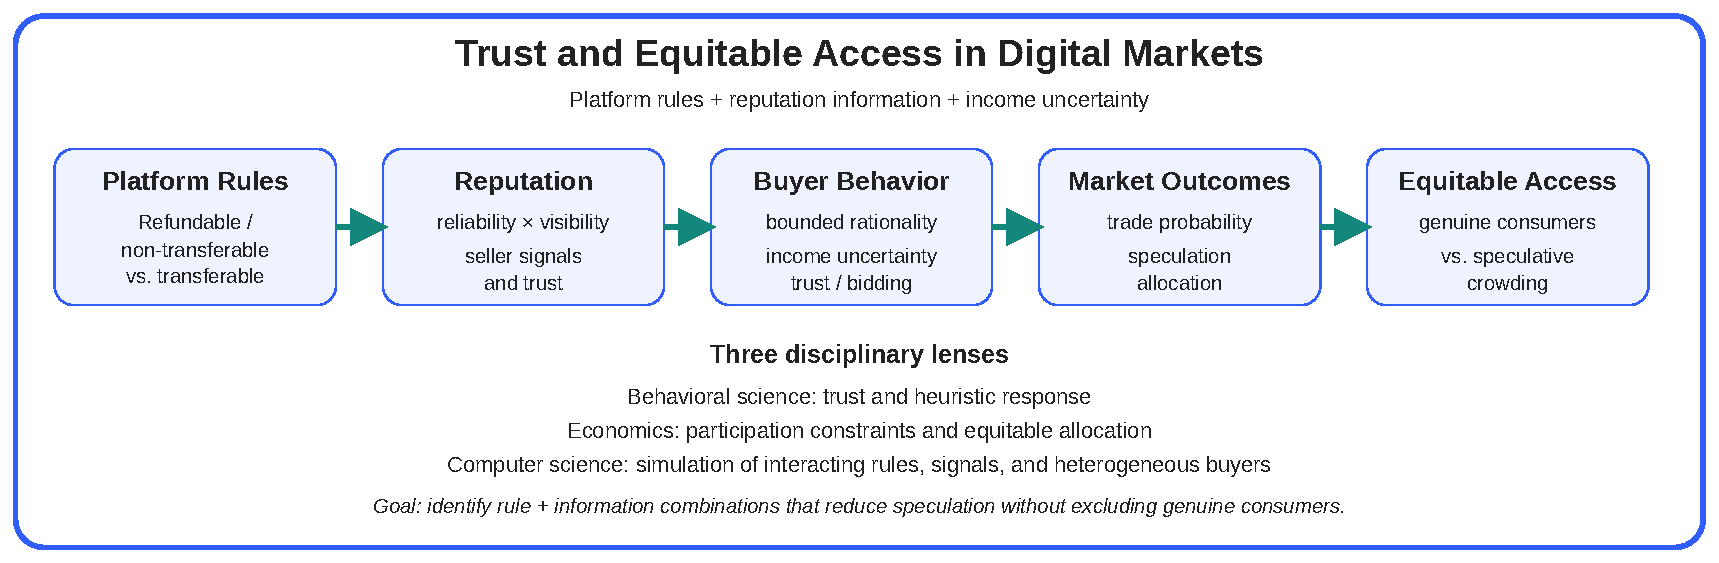
\includegraphics[width=\textwidth]{figures/ps1_teaser.pdf}
\caption{Proposed digital-market mechanism: platform rules and reputation information shape buyer behavior under income uncertainty, which in turn affects speculation and equitable access to scarce goods.}
\Description{A five-part flow connects platform rules and reputation information to buyer trust and bidding, market allocation, speculation, and equitable access, with income uncertainty moderating participation.}
\label{fig:teaser}
\end{teaserfigure}
\maketitle\raggedbottom\coursemeta

\section{Three connected research questions}
Digital markets let strangers transact despite incomplete information, but the same platform design that improves trust may also shape who receives scarce opportunities. Building on reputation research~\cite{tadelis2016,zloteanu2018}, I study the joint effects of reputation information, platform rules, and income uncertainty. \textbf{Q1---Economics:} How does income uncertainty affect consumers' ability to benefit from apparently open digital-market access? \textbf{Q2---Computation:} Which combinations of platform rules and reputation signals reduce speculative crowding while preserving access for genuine consumers? \textbf{Q3---Behavior:} How does the amount and visibility of reputation information change trust and willingness to transact under financial uncertainty? The questions are interdependent: behavioral responses determine demand, economics evaluates allocation and welfare, and computation makes alternative mechanisms comparable at scale (Fig.~\ref{fig:teaser}).

\section{Answer to Q1: incentives and intellectual lineage}
I inherit from Tadelis~\cite{tadelis2016} the economic role of reputation in reducing information frictions between strangers. I extend this framework by treating financial capacity as a second source of uncertainty: consumers may have market access without having the liquidity to use it. My hypothesis is that income uncertainty tightens participation constraints and can shift scarce goods toward financially secure or speculative buyers even when transaction costs are low. The economic outcome is therefore not only trade, but the distribution of opportunities and surplus across buyer types. This creates a tension with the usual efficiency goal: a rule can improve allocation or transaction completion while making access less equitable.

\section{Answer to Q2: method and evaluation}
I represent the market with heterogeneous buyer agents competing for scarce goods. The baseline compares two institutional rules---\emph{refundable but non-transferable} versus \emph{transferable but non-refundable}---while varying demand, scarcity, speculative participation, income uncertainty, and reputation-signal reliability/visibility. The model records purchase probability, speculative activity, buyer surplus, and access by financially constrained versus unconstrained consumers. A smallest factorial check compares the two rules under low/high demand and low/high speculation; a meaningful extension varies reputation visibility. The computational goal is not to predict a real platform from synthetic data, but to make the mechanism transparent, reproducible, and falsifiable. Actual outputs will be reported only from the verified notebook; other outcomes remain planned.

\section{Answer to Q3: behavior and competing explanations}
I inherit from Zloteanu et al.~\cite{zloteanu2018} the finding that trust and reputation information influence judgments of unfamiliar users. I advance it by testing whether information affects \emph{action}, not only judgment, when financial constraints are present. One hypothesis is a non-linear trust response: insufficient reputation information may suppress transactions, while highly salient positive reputation may encourage heuristic reliance and speculative bidding. A competing explanation is a liquidity channel in which income risk lowers willingness to pay regardless of reputation. A discriminating experiment varies reputation visibility while holding seller quality fixed and compares high- and low-income-risk buyers. The proposed evidence cannot establish population-level causal effects without larger human-subject or field data.

\section{Advanced development and future directions}
The long-run contribution is a design framework for trustworthy and equitable digital markets that integrates behavioral responses, economic participation constraints, and computational mechanism design. Akerlof's Nobel-recognized work establishes why information asymmetry can undermine exchange~\cite{akerlof1970,nobel_akerlof}; Simon's bounded-rationality work and Turing Award recognize decision-making and computational perspectives~\cite{simon1955,simon1978,simon_turing}. I retain their enduring questions of trust and rational decision-making but advance the boundary to platforms where algorithms control information visibility and transaction rules at scale. The key synthesis is that improving trust is not sufficient if the same information or rules concentrate opportunities.

\begin{table}[h]
\caption{Roadmap from foundations to the 2056 contribution.}
\begin{tabularx}{\columnwidth}{@{}p{1.45cm}Y@{}}\toprule
\textbf{Horizon}&\textbf{Milestone and evidence}\\\midrule
Foundation&Akerlof: information asymmetry; Simon: bounded decision-making and computational support.\\
PS1&Reproduce the baseline mechanism and compare rule--information treatments.\\
Next study&Test reputation response against the competing liquidity explanation with heterogeneous buyers.\\
Longer term&Validate the mechanism with human participants and platform/ticketing data.\\
2056&Design scalable rules and reputation systems that preserve trustworthy exchange without crowding out genuine consumers.\\
\bottomrule
\end{tabularx}
\end{table}

\noindent\textbf{Expected 2056 Nobel Prize and Turing Award contribution statement.}
By 2056, I aspire to contribute a theory and computational design framework for trustworthy and equitable digital markets, addressing trust, allocation, and participation under uncertainty. By integrating behavioral science on reputation responses, economics of financial constraints and allocation, and computer science simulation of platform mechanisms, I aim to identify designs that reduce speculation while preserving genuine access. Progress will be demonstrated through reproducible computation, behavioral tests, and field validation.

\subsection*{Open Science Statement}
\textbf{GitHub:} \url{https://github.com/ixs3v3n/PS1-Xuantong}\\
\textbf{Google Colab:} \url{https://colab.research.google.com/drive/193R57-a-d-1RZOn3iszmP1Ya4X1AoBF2}\\
The release will contain the simulation code, dependencies, parameter settings, synthetic inputs, and actual outputs required to reproduce the computational analysis.

\subsection*{Statement of Contribution to the UN's SDGs}
\textbf{Hugging Face:} \url{https://huggingface.co/spaces/dku-comsci-econ206-2026/Xuantong_Fu_Space}\\
The open-access interactive game supports \textbf{SDG 4---Quality Education}~\cite{sdg4} by allowing learners to interact with the same reputation-information trade-off studied in the proposal. The tool is an educational artifact; learning gains remain to be evaluated.

\clearpage\nobalance
\section*{Author Notes}
\subsection*{Acknowledgements}
I thank Prof. Luyao Zhang, Program Chair, and Prof. Ken Rogerson, Program Discussant, of the \emph{2056 Nobel and Turing Laureate Program Launch Workshop}, held September 7, 2026 at Duke Kunshan University. I also thank Jiayang Sun and Zhenning Wang, my teammates in Week 3 session A, and the COMSCI/ECON 206 class for discussion and feedback. I am responsible for the proposal and remaining errors.
\subsection*{Individual contribution}
I developed the research question, interdisciplinary mechanism, proposal, computational design, and learning-tool concept. Any shared material or feedback is identified where used.

\bibliographystyle{ACM-Reference-Format}
\bibliography{references}

\appendix
\section{Technical details and reproducibility}
\textbf{Links and version.} Hugging Face: \DemoLink. GitHub: \GitHubLink. Colab: \ColabLink. Author: Xuantong Fu. Tested: [date], version [version/commit].

\textbf{Mechanism.} Buyers face scarce goods under two rules: refundable/non-transferable versus transferable/non-refundable. Agents differ in income uncertainty and speculative participation. Reputation signals vary in reliability and visibility. Outcomes are purchase probability, surplus, speculation, and access by buyer type. The simulation resets from a documented parameter file and uses fixed seeds where stochasticity is introduced.

\textbf{Compact rule.} For each treatment: initialize heterogeneous buyers and scarce supply $\rightarrow$ reveal rule and reputation information $\rightarrow$ buyers choose/submit bids or purchase decisions $\rightarrow$ allocate goods $\rightarrow$ record purchase, surplus, speculation, and access $\rightarrow$ repeat across demand/scarcity conditions.

\textbf{Checks.} Boundary: zero speculative buyers and minimum demand. Typical: baseline demand, scarcity, and mixed buyer types. Invalid input: negative demand or an income probability outside $[0,1]$; the implementation rejects or normalizes invalid values rather than silently treating them as valid. Results from the Week 2 browser prototype are reported separately from future simulation results.

\textbf{Responsible boundary.} The learning demo uses a static browser implementation only: no Hugging Face CPU/GPU runtime, backend, database, secret, API call, or paid service. Checks include desktop/mobile layout, keyboard interaction, readable labels, reset behavior, and invalid-input handling. Privacy is not collected or stored. Population-level behavioral claims remain unverified until larger experiments are conducted.

\section{AI-assistance statement}
I used ChatGPT (GPT-5.6 Luna) during September 2026 for bounded support with proposal structure, wording, computational-design discussion, and debugging of the browser prototype. I retained responsibility for the research question, disciplinary integration, hypotheses, treatment conditions, outcome measures, and final decisions. AI suggestions were treated as drafts: alternatives that were too broad, unsupported, or inconsistent with the intended mechanism were rejected or revised. I checked code behavior by running the game and checking transitions, locked choices, reset behavior, boundary/invalid inputs, and displayed calculations. I checked academic claims against the original papers and kept synthetic or pilot outputs separate from planned findings. AI output was not used as scholarly evidence.

\section{Cumulative Intellectual Development}
This proposal develops my Intellectual Statement II through the \emph{2056 Nobel and Turing Laureate Program Launch Workshop}, September 7, 2026, Duke Kunshan University, IB 2050. Program Chair: Prof. Luyao Zhang. Program Discussant: Prof. Ken Rogerson. My session: A. Rethinking Reputation in Online Marketplaces. My role: Behavioral Scientist. My teammates: Jiayang Sun, Zhenning Wang.

The earlier project focused mainly on how reputation information changes trust and transaction decisions. Peer discussion and field evidence motivated a broader question: trust is valuable, but platform rules and financial constraints can determine who actually receives scarce opportunities. I therefore added income uncertainty, speculation, and ticketing rules, changing the project from a reputation-only problem into a joint trust-and-access problem. [Add the exact dated peer comment and its source before submission.]

\section{Field and open-source inspiration}
The \emph{Joint Interdisciplinary Field Trip---Technology, Computation, Culture \& Society in Action} took place September 4, 2026. The field evidence includes the Tencent Shanghai Office green-cloud-computing exhibit and the Shanghai Science and Technology Museum four-axis trainer. The photographs are retained with their captions and alt text from Week 2. The Tencent exhibit directly showed energy-efficiency and renewable-energy measures; my interpretation is that computational systems can change resource allocation at organizational scale. The museum exhibit directly showed an interactive aerospace-motion experience; my interpretation is that information and technology are partly effective through how people experience and understand them.

The Week 2 open-source tools were Microsoft Recommenders and the CDC Measles Outbreak Simulator. Microsoft Recommenders motivated the partner-ranking/opportunity-concentration perspective; its recommendation focus limits direct transfer to the marketplace mechanism. The CDC simulator motivated interactive comparison of intervention conditions; its disease-specific assumptions limit direct transfer to market behavior. Official links, repositories, licenses, versions, and access dates are retained in the Week 2 supporting materials.

\section{Review response and revision record}
\textbf{Strength retained:} the proposal keeps a concrete platform setting and a clear interdisciplinary mechanism.\\
\textbf{Constructive concern addressed:} [insert actual peer criticism] led me to [insert actual revision].\\
\textbf{Question clarified:} [insert actual peer question] led me to specify [mechanism, variable, or test].\\
Future peer-review results will be added without replacing earlier versions.

\clearpage\onecolumn
\section{Structured abstract and cumulative proposal map}\label{app:abstract}
\begin{table}[H]
\caption{Cumulative proposal map.}
\label{tab:abstract-map}
\renewcommand{\arraystretch}{1.18}
\begin{tabularx}{\textwidth}{@{}p{0.27\textwidth}Y@{}}
\toprule
\textbf{Proposal element} & \textbf{Current statement / change} \\
\midrule
Background & Digital markets reduce transaction frictions, but reputation, rules, and financial constraints can jointly shape trust and access. \\
Motivation and application & Scarce goods create a joint problem of information design, speculation, platform rules, and unequal purchasing capacity. \\
Three connected questions & Economics studies income constraints; computation compares rule--signal combinations; behavior studies trust and action under uncertainty. \\
Method and model assumptions & Heterogeneous-agent simulation with two ticketing rules, variable demand/scarcity/speculation, and reputation conditions. \\
Results or expected results & The Week 2 game provides preliminary observed outputs; PS1 simulation results remain planned until reproduced in the notebook. \\
Intellectual merits & The synthesis asks when information that improves trust can nevertheless worsen equitable access. \\
Practical impacts & The framework can inform platform/ticketing design, while the open-access game supports SDG 4 learning. \\
Feedback received and revision made & The project expanded from reputation-only decisions to the interaction of reputation, platform rules, speculation, and income uncertainty. \\
\bottomrule
\end{tabularx}
\end{table}

\end{document}
